\documentclass[../main.tex]{subfiles}
\graphicspath{{\subfix{../images/}}}
\begin{document}
\textbf{PACE}

{\small In the morning, before or after breakfast, in school (before  classes, after breaks, before the afternoon program or tests) or when you have a challenging task ahead of you.

%\vspace{5mm}
\noindent
\begin{tabular}{p{2cm} p{10cm}}
    \raisebox{-0.8\totalheight}{  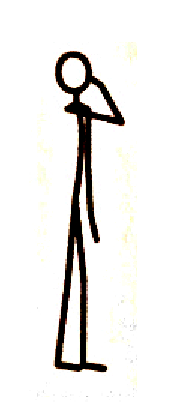
\includegraphics[width=1.1cm]{water} }
  &
    \textbf{Drink Water:} 
    Water is an excellent {conductor} for electrical energy.
    An optimal learning performance requires our {hydration levels} to be {balanced}.
    The water balances allows the {efficient storage and retrieval of information} in the brain and in the body
    and activates {optimal electrical and chemical processes} between the brain and the nervous system.\\

  \raisebox{-1.2\totalheight}{  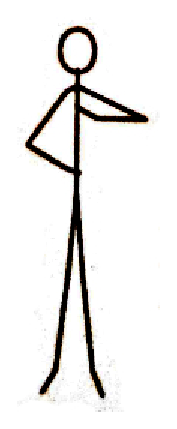
\includegraphics[width=1.1cm]{buttons} }
  &
    \textbf{Brain Buttons:}
Hold one {hand over the belly button} or massage a big area,  the other hand massages the {points underneath the collarbone}, immediately left and right of the sternum on the first rib.
According to acupuncture, these are the end points of the kidney meridian\footnote{energy pathway in our body)}.
\begin{itemize}[noitemsep]
	\item The hemispheres of the brain get centered and energetically charged.
	\item The perception of the surroundings is sharpened.
	\item Improves your awake state.
	\item Hand--eye coordination improves.
	\item Getting up in the morning gets easier, if done beforehand.
\end{itemize}
  \\
    \raisebox{-0.9\totalheight}{  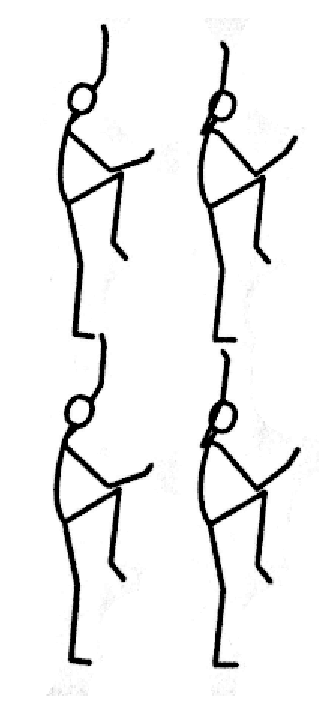
\includegraphics[width=2.4cm]{crossover} }
  &
    \textbf{Crossover Movement:} {{Cross over 10 times}} (alternating: right elbow to the left knee and then left elbow to the right knee, 5 times each)
    while keeping your head steady and having the {eyes in the upper left corner}.
{{Same side 10 times}} (right elbow to right knee alternated with other side, 5 times each) {eyes in the lower right corner}.
{{Alternating:}} 1 time cross over, each direction once, eyes left up. 1 time same side, each side once, eyes down right. Repeat this 4 times, gives 16 movements.
 
{{Possible progression:}} Add 16 times cross over with eyes closed.
\begin{itemize}[noitemsep]
	\item Optimizes attention, awareness and perception.
	\item Language and expression become clear (especially while reading and at orthography).
	\item Eye and ear energy get balanced.
\end{itemize}
  \\
    \raisebox{-1.2\totalheight}{  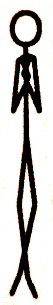
\includegraphics[width=0.5cm]{Hookup} }
  &
    \textbf{Hook Ups:} Stand with {legs crossed}, left over right, {cross the arms} over in front of your body, interdigitate (interlock) your hands and bring them {in front of your sternum}. Push the tongue flat against the roof of your mouth.

   
\begin{itemize}[noitemsep]
\item The meridians get connected and activated.
	\item The emotions in the limbic system get connected to reason in the neocortex area.
	\item Stimulates learning.
	\item Stimulates effective action.
	\item Centring, ex. during (or better before) an argument, bad feelings, ADHS, $\ldots$
\end{itemize}

  \end{tabular}
}
\end{document}